\documentclass{aes2e}

% PACKAGES
\usepackage{gensymb}
\usepackage{textcomp}
\usepackage{array}
\usepackage{graphicx}

% Graphics Path
\graphicspath{{images/}}

% Metadata Information
\jyear{2018}
\jmonth{?}
\jvol{1}
\jnum{1}


\begin{document}

\title{Immersive Audio Recording for Virtual and Augmented Reality}

\authorgroup{
\author{Lewis Thresh},
\role{Research Technician},
\author{Hasham Riaz},
\role{Abbey Road Studios}
AND \author{Gavin Kearney},
\role{Senior Lecturer}
\email{(lewis.thresh@york.ac.uk)\quad\quad\quad\quad\quad(Hasham.Riaz@abbeyroad.com)\quad\quad\quad\quad\quad\quad (gavin.kearney@york.ac.uk)}
\affil{University of York, York, UK}
\affil{Abbey Road Studios, London, UK}
}

\abstract{}

\maketitle

\section{INTRODUCTION}
	% Introduce the concept of recording/mixing music for VR and the differences between thsi and recording/mixing in stereo. 
	This work follows on from \cite{riaz2017multichannel}...

\section{Recording at Abbey Road Studios}
	% - Description of recording process
	% - Band + song
	% - List of microphones arrays + positions

\section{Test Material Preperation} % Think of a better heading
	\subsection{Video}
		As two different 360\textdegree cameras were used during recording, two different methods of spherical video encoding were used. \textbf{[Look at has's AES/thesis for this?]}

			\subsubsection{Position A - 360\textdegree perspective}
				Writing

			\subsubsection{Position B - 180\textdegree perspective}

	\subsection{Audio}
		% - Mixing of spots
		% - Position Encoding
		% - Array processing
		% - Spot mic / array encoding
		% - Binaural decoding		
		% - Reaper project layout
		% - Ambix plugins

		% - Video encoding
		% - Head/soundfield rotation integration
		% - Different viewing angles / different encoding

\section{Listening Tests}
	% Describe the listening test process

	Two rounds of listening tests were conducted for viewing position A (test 1) and B (test 2). The procedure was identical however the data used, such as video and microphone configurations used were different for each. Both tests recruited participants both from the University of York and Abbey Road Studios. All participants were required to have some previous experience with mixing/producing and/or spatial audio. The number of participants recruited for each test were as follows:

	% Table of number of participants
	\begin{center}
		\begin{tabular}{|r |c c|} \hline
			Recruted From & Test 1 & Test 2 \\ \hline
			UoY & 15 & 29 \\
			Abbey Road & 4 & 9 \\ 
			\textbf{Total} & \textbf{19} & \textbf{38} \\\hline
		\end{tabular}
	\end{center}

	\subsection{Attributes Focus Group}
		The aim of the listening test was to assess the performance of each microphone array configuration for a VR environment in terms of its spatial and timbral quality. Due to the subjectivity of such a test, a focus group was assembled with the purpose of producing a list of mutually agreeable adjectives to use to describe certain spatial and timbral attributes. The attributes chosen to use within the listening tests are shown in table\ref{table:attTable}. \\

		% Table of Spatial and Timbral attributes
		\begin{table}[h]
			\begin{tabular}{m{2.2cm} | m{0.31\textwidth}}
				\textbf{Attribute} & \textbf{Description} \\ \hline
				\multicolumn{2}{l}{\textbf{Spatial}} \\ \hline
				Locatedness & How easily you can locate a sound source within the VR environment \\
				Sense of Space & How well the space where the recording was made is perceived \\
				Externalisation & Perception of sound coming from all around your head \\
				Envelopment & Whether the sounds are perceived to originate inside of outside of the head \\ \hline
				\multicolumn{2}{l}{\textbf{Timbral}} \\ \hline
				Full & Abundance of low frequencies present \\
				Bright & Abundance of high frequencies present \\
				Flat & Lack of high and low frequencies present \\
				Rich & The mix sounds good with both high and low frequencies \\
				Realistic & The sounds heard in the VR experience are realistic (sound like real instruments) and timbral characteristics have been preserved. \\
				Loud & The perceived level sounds high
			\end{tabular}
			\caption{Table of Spatial and Timbral Attributes}
			\label{table:attTable}
		\end{table} 
			

	\subsection{Procedure}

		Participants was asked to wear and Oculus Rift DK2 headset and a pair of Audio Technica MH50x headphones and watch the first 80 seconds of the chosen take from their respective positions (A or B). Once the clip was finished participants would answer a questionnaire. This involved rating on a scale of 1 - 10 the level at which they experienced each of the spatial attributes listed in table \ref{table:attTable} and to list any timbral attributes they felt best described the timbre of the recording. 

		To ensure that all participants understood each of the attributes in the same way a short training exercise was conducted before each test. This involved taking the participants through each of the attributes with audio examples. 


\section{Analysis}
	% Analysis 1 - 5
	To best analyse the results, five analysis targets were defined:

	\begin{tabular}{r p{5.5cm}}
		Analysis 1: & Does viewing position effect Spatial Attribute rating? \\
		Analysis 2: & Does the choice of microphone array effect Spatial Attribute score? \\
		Analysis 3: & What is the effect of using Directional or Diffuse-Field Arrays? \\ 
		Analysis 4: & Is there a correlation between SA score and selected timral attributes? \\
		Analysis 5: & Is there a in perception of timbre with difference viewing positions?
	\end{tabular}

	\subsection{Analysis 1: Does viewing position effect spatial attribute scores?}

		To assess the potential effect of viewing position on spatial attribute score, data was grouped into 8 sections: An average score for each spatial audio attribute (4 groups) each split into the average score for viewing position A and B (8 groups) illustrated in figure \ref{image:AvsB}.

		\begin{figure}
			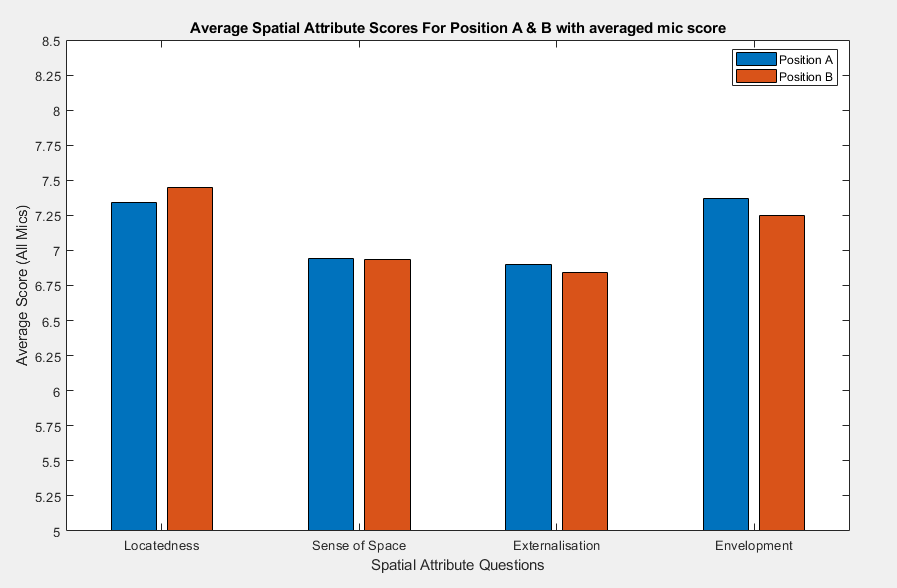
\includegraphics[width=0.5\textwidth]{AvB_Bar.PNG}
			\caption{Bar chart showing average spatial attribute score for each spatial attribute at viewing position A and B}
			\label{image:AvsB} 
		\end{figure}

		
		




	\subsection{Analysis 2: Does the choice of microphone array effect Spatial Attribute score?}


	\subsection{Analysis 3: What is the effect of using Directional or Diffuse-Field Arrays?}


	\subsection{Analysis 4: Is there a correlation between SA score and selected timral attributes?}


	\subsection{Analysis 5: Is there a in perception of timbre with difference viewing positions?}



\bibliographystyle{aes2e}
\bibliography{aes2e}

\end{document}
